

\chapter{An Overview of MPTCP} \label{chap:mptcp}
Multipath TCP is an extension of the TCP protocol which was published as an Experimental standard by the Internet Engineering Task Force (IETF) in RFC 6824 \cite{rfc6824} in January 2013. Several implementations have since been developed. This work was done using version 0.89 of the Linux Kernel implementation \cite{mptcp} . At its core, MPTCP aims to allow a host to use multiple link-level paths for a single TCP connection, improving throughput and redundancy.\\

This section will cover how the MPTCP protocol works by explaining which types of packets are sent, and how the different parts of a connection are performed.

\section{General Operation and Option Types}
MPTCP initially behaves like a regular, single TCP connection. However, once the use of MPTCP has been successfully negotiated, either one of the hosts can decide to start a new TCP connection that will join the MPTCP connection. Figure \ref{pic:mp setup} shows how two hosts can use the protocol to setup several subflows. The host can then use all the individual TCP connections (called subflows) to spread the data, using the combined bandwidth of each path.\\

\begin{minipage}[c]{\textwidth}
\centering
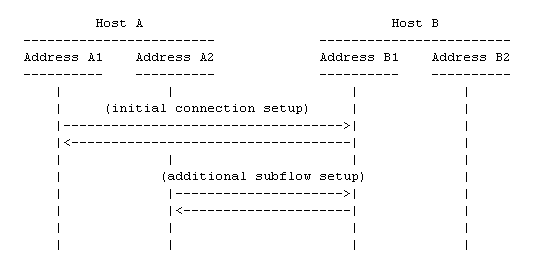
\includegraphics[scale=0.6]{Figures/mptcpsetup.png}
\captionof{figure}{Setting up multiple subflows between two hosts}
\label{pic:mp setup}
\end{minipage} \\

MPTCP's operation is based on the use of TCP options. The protocol uses the option kind 20, which is reserved by the Internet Assigned Numbers Authority (IANA). The option has a varying length which will be discussed in further detail later. The first four bits of an MPTCP option are always used to indicate the option subtype which is one of the eight following values:

\begin{itemize}
\item Subtype 0, MP\_Capable: used to negotiate the use of MPTCP during the establishment of the first TCP connection.
\item Subtype 1, MP\_Join: used during the establishment of a secondary TCP connection to signal that it is a subflow of an existing MPTCP connection.
\item Subtype 2, DSS: contains the data sequence mapping used to indicate how data from different subflows is ordered, enabling re-assembly on the receiver side.
\item Subtype 3, Add\_Addr: used within a subflow to signal the existence of other addresses that can be used to setup additional subflows.
\item Subtype 4, Remove\_Addr: used like Add\_Addr, but to signal that an address is no longer available.
\item Subtype 5, MP\_Prio: addresses can be used as either normal subflows or backup. This subtype allows a host to change to status of an address to and from backup.
\item Subtype 6, MP\_Fail: this option is used to close a subflow which has been opened correctly but within which modifications to the data have been detected. If the data sequence mapping is modified, the data on that subflow cannot be used since the re-assembly will fail. The connection is therefore closed using an MP\_Fail option which allows the host to ``forget'' all the data that was sent on that subflow.
\item Subtype 7, MP\_Fastclose: in an MPTCP connection, a TCP rst will only close that particular subflow. This option subtype is equivalent to an rst, but for the whole MPTCP connection.
\end{itemize}

The format of each MPTCP option as defined in the RFC can be found in appendix \ref{append:mp opt format}. A given packet can contain multiple MPTCP options. Typically, Add\_Addr options can be piggy-backed onto data packets which also contain the DSS option.\\

We will now go over how the important steps of an MPTCP connection are performed. For a more detailed explanation, please consult RFC 6824.\\ \\



\section{First Connection Establishment}
When a host A wishes to establish an MPTCP connection with a host B, it will begin by initiating a TCP connection, where the first SYN packet will contain an MP\_Capable option. This option contains the MPTCP version number, a number of flags which are used to negotiate the cryptographic algorithms to employ, and the 64-bit key which A will use for this connection (the whole MPTCP connection, not just the subflow). \\

B will then reply with a SYN+ACK. If the packet does not contain the MP\_Capable option, then either the host cannot use MPTCP, or the options have been removed along the way. In any case, the connections reverts to standard TCP. If the option is present, it will contain the key that B will use. Host A responds with the final ACK packet, completing the three-way handshake. This ACK must also contain an MP\_Capable option, along with both host's keys. \\

Each host can then compute the tokens that will uniquely identify the connection on each host. Theses tokens are 32-bit values computed by truncating a hash of the key to its most significant 32 bits. A token must be unique for a given host. Figure  \ref{pic:mpcapex} shows the packets exchanged during this process.

\begin{figure}[!t]
\centering
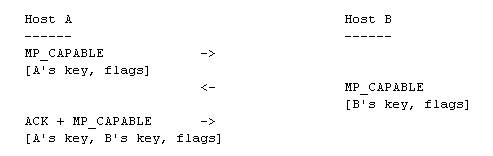
\includegraphics[scale= 0.6]{Figures/mpcapex.png}
\caption{Data exchanged for MPTCP connection setup}
\label{pic:mpcapex}
\end{figure}

\section{Advertising New Addresses}
Once a connection is established, each host may wish to indicate to the other that it has additional addresses available for new subflows. To do this, it will use an existing subflow and send a packet with the Add\_Addr option (as mentioned earlier, this can be piggy-backed onto a data packet). The address is mapped to an Address ID which is unique per host and per connection (the address for the original subflow has the ID 0). The wishing to advertise a new address will therefore send its address along with the ID so that the other host can know the mapping. MPTCP supports both IPv4 and IPv6 addresses. \\

If an address later becomes unavailable, the host can send a Remove\_Addr option to signal that the other host should no longer attempt to connect to it. Remove\_Addr exclusively uses the Address ID to reference an address. \\

Finally, as mentioned earlier, addresses can be used as regular or backup addresses. If a host wishes to indicate that an address should be used as backup (or that a backup address can now be used regularly), it can send an MP\_Prio option. This option references the address in question by its ID, and contains a single bit which indicates the address' new priority.

\section{Joining an Existing Connection}
If host A wants to start a new subflow for the MPTCP connection, it will send a SYN packet to one of host B's advertised addresses (see section \ref{add adv}). This SYN will contain an MP\_Join option. The MP\_Join option contains the token to identify which MPTCP connection it concerns, as well as the Address ID of the packet's source (in case the actual header is modified). Letting just any other TCP flow join an ongoing connection would allow attackers to join it and disrupt the communication. Therefore, the join procedure uses an authentication method/ To this end, the SYN also contains a 32-bit random number. \\

Host B will reply with a SYN+ACK containing its own random number. It will also have to use both keys that were exchanged to compute a HMAC of both random numbers. Due to option space limitations, it can only send a truncated (64 bits) version of this HMAC to host A. Unlike MP\_Capable, if the SYN+ACK does not contain an MP\_Join option, the TCP connection is closed. \\

Host A must verify that the HMAC is correct. If it is, its own HMAC (in full this time, since no other data is needed) to host B. Even though the three-way handshake has thus been completed, host B must still verify host A's HMAC and will close the connection if it is wrong (with an rst). Figure  \ref{pic:mpcapex} shows the packets exchanged during this process.

\begin{figure}[!t]
\centering
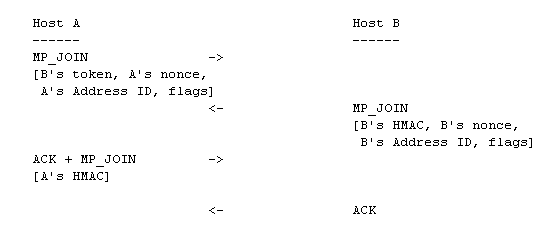
\includegraphics[scale= 0.6]{Figures/mpjoinex.png}
\caption{Data exchanged for MPTCP JOIN}
\label{pic:mpjoinex}
\end{figure}

\section{Sending Data}
Data packets belonging to an MPTCP connection will contain a DSS option. This option contains the equivalents of TCP sequence numbers and acknowledgments, but over all the subflows of the MPTCP connection. The Data Sequence Number, Subflow Sequence Number and Data-Level Length allow the receiver to re-order the packets coming from multiple TCP connections into a single coherent data stream. The data sequencing mapping will be discussed in more detail when we will cover reassembly. \\

DSS options also contain the DATA\_FIN flag, which is used to indicate that a host has no more data to send. This flag functions like the TCP FIN flag for the entire MPTCP connection and is the regular way of closing the connection.

\section{Fastclose and Failure}
In regular TCP, a host can rapidly close a connection by sending an rst. For MPTCP, a host must close multiple TCP connections to stop a single MPTCP connection. To do this, host A will send an MP\_Fastclose option on one of the subflows, along with host B's key. Host A will also send a TCP rst on each one of the other TCP subflows (leaving only one active subflow on the MPTCP connection). If host B recognizes the key, it will answer by closing down the final subflow with an rst. \\

If a subflow proves unsuitable for MPTCP (for example, if a middle bow is modifying the payload and making the correct data sequence mapping irrecoverable), the subflow will be closed with an MP\_Fail option. This option indicates the Data Sequence Number before any data was sent on that subflow, allowing the receiver to discard any corrupt information the subflow could have sent.
